\documentclass{article}
\usepackage[utf8]{inputenc}
\usepackage{graphicx}
\graphicspath{ {./images/} }
\usepackage{amsmath}
\usepackage{hyperref}
%\usepackage[english]{babel}

\usepackage[left=2cm,right=1cm, top=2cm,bottom=2cm,bindingoffset=0cm]{geometry}

\renewcommand{\normalsize}{\fontsize{14}{18pt}\selectfont}

\title{ Detection of the rare variants for analyzing hemagglutinin genes     }
\author{ Ignat Sonets, Kamilla Faizullina}
\date{\empty}
 
\begin{document}


\maketitle
We analyze the amplicon data to detect rare variants. As occuring errors exist, we use three control sequences to understand which variants are real and which of them was detected as mutation due to error. 
\section{Introduction}
Vaccine is a formulation of killed or attenuated pathogens, or antigens derived from them which help prevent, ameliorate, or treat infectious disease by stimulating antibody production or cellular immunity against the pathogen \cite{vac}. Epitope is a molecular region, usually an amino acid sequence, on the surface of an antigen that is capable of eliciting a specific immune response. \cite{epit}. Any changes of epitopes lead to decreasing efficiency of antibodies. 

Influenza viruses are important human respiratory tractpathogens responsible for the seasonal epidemics andsporadic pandemics around the world \cite{hv} Influenza exists as quasispecies. Quasispecies are  viral variants leading to diversification of the original strain \cite{quas}. Deep sequencing enables us to study  mixed populations. However, the detection of rare varints might be challenging due to errors which accure prior to or during sequencing. 


\section{Methods}
\subsection{Data}
In order to analyze the hemaaglutinin genes, we use Amplicon of H3N2 HA infecting Homosapien labeled SRR1705851 from The National Center for Biotechnology Information database \cite{ncbi}. We analyze the quality of the amplicon data via Fastqc \cite{fc}. Figure 1 illustrates the quality of this sequencing data. It is quite good and we do not need to filter the reads. We use the reference data \cite{ref}. Also, we use three control sequencing data labeled  SRR1705858, SRR1705859 and SRR1705860 \cite{control}. 
 

\subsection{Methods}
In order to to map the data from the resistant strain to the reference sequence, we use the aligner called BWA-MEM \cite{bwa}.  VarScan is used to find SNP \cite{var}.


\begin{figure}[h]
\centering
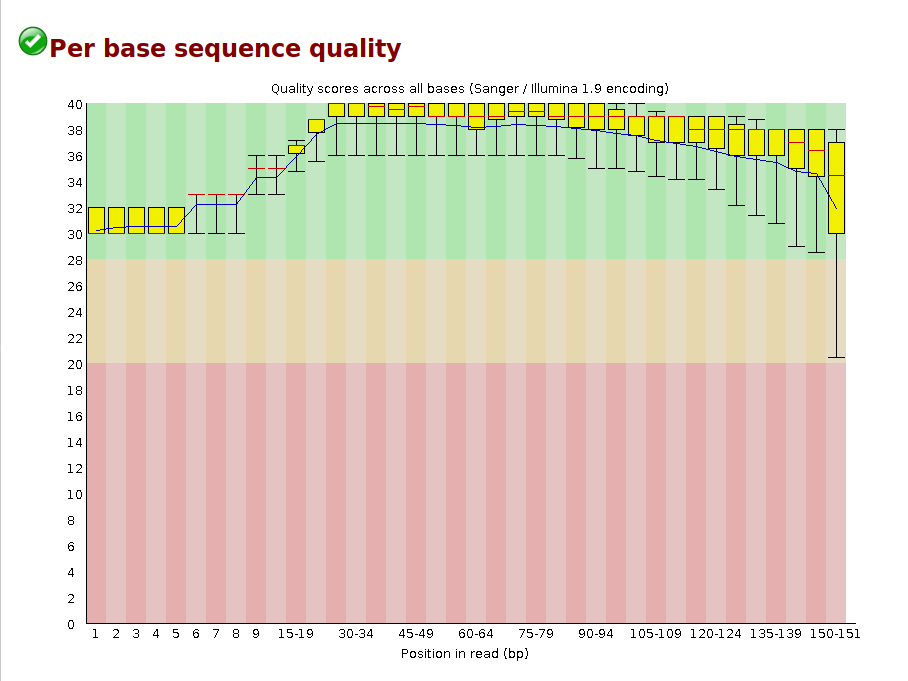
\includegraphics[scale=0.35]{data_q.png} 
 
\caption{ The quality of the sequence labeled SRR1705851  }
\label{saw}
\end{figure}

\section{Results}

	\begin{table} 
	\centering
	\begin{tabular}{|c|c|c|c|}
		\hline
		The sequence & Reads & Mapped \\
		\hline
		SRR1705851 & 358265 & \\
		\hline
		SRR1705858 & 256586 & \\
		\hline
		SRR1705859 & 233327 & \\
		\hline
		SRR1705860 & 249964  & \\
		\hline
	\end{tabular}
\caption{Data}
\end{table}
 
\subsection{Common variants}
The  data labeled SRR1705851 is used to detect the variants.  The parameter --min-var-frequency equals 0.95 for searching common variants. Five SNPs were reported (Table \ref{tab:vars}). We used the codon table to check if these mutations can affect the protein, but all these variants do not change the amino acids. 


\begin{table}
	\centering
	\begin{tabular}{|c|c|c|c|c|}
		\hline
		Position & Ref  & Alt & Triplets & Amino acids\\
		\hline
		72 & A & G & ACA $\rightarrow$ ACG & Threonine $\rightarrow$  Threonine \\
		\hline
		117  & C & T & GCC  $\rightarrow$  GCT & Alanine $\rightarrow$  Alanine\\
		\hline
		774  & T & C & TTT $\rightarrow$   TTC & Phenylalanine $\rightarrow$  Phenylalanine\\
		\hline
		999  & C & T & GGC  $\rightarrow$  GGT & Glycine $\rightarrow$  Glycine \\
		\hline
		1260 & A & C & CTA  $\rightarrow$  CTC & Leucine $\rightarrow$  Leucine \\
		\hline
	\end{tabular}
	\caption{ The variants, --min-var-frequency=0.95 }
	\label{tab:vars}
\end{table}

%These SNPs do not cause any changes. 

\subsection{Rare variants}
 Next, we run VarScan to detect rare parameters, but --min-var-frequency equals 0.001. We obtained 21 SNPs. To find the difference between real rare variants and possible sequencing error, we use three isogenic viral samples. Again, we align these samples to the reference and get SNPs.  Table\ref{tab:freqs} presents the mean and standard deviation for frequencies of detected variants. Table \ref{tab:rarevars} presents the rare SNPs with frequencies that are more than 3 standard deviations away from the averages in the reference results. 
 
   %Two SNPs are detected (Table 2). These parameter was the same for three control sequences. 



\begin{table} 
	\centering
	\begin{tabular}{|c|c|c|c|}
		\hline
		The control sequence & Mean frequency & Standard deviation  \\
		%\hline
		%SRR1705851 & 358265 & \\
		\hline
		SRR1705858 & 0,24928571 & 0,04716921734 \\
		\hline
		SRR1705859 & 0,2369230769 & 0,05237640771 \\
		\hline
		SRR1705860 & 0,25032787 & 0,07803775183 \\
		\hline
	\end{tabular}
	\caption{Data}
	\label{tab:freqs}
\end{table}

\begin{table}
	\centering
	\begin{tabular}{|c|c|c|c|c|}
		\hline
		Position & Ref  & Alt & Triplets & Amino acids\\
		%\hline
		%38 & T & C & CTG  $\rightarrow$  CCG  & Leucine $\rightarrow$  Proline \\
		\hline
		307  & C & T & CCG  $\rightarrow$  TCG &  Proline $\rightarrow$ Serine \\
		\hline
		1458  & T & C & TAT $\rightarrow$   TAC &  Tyrosine $\rightarrow$ Tyrosine  \\
	 
		\hline
	\end{tabular}
	\caption{ The rare variants,  }
	\label{tab:rarevars}
\end{table}

\section{Discussion}
% In first experience, four varians were found, however, all of them does not change anything. \\ The variant which position is 307 detected in second experience replace one aminoacid with other. This position is included in the epitope region \cite{mun}. There are wayes to avoid errors which could be detected as mutations.  For example, repeat analysis  and use control data. 
%\section{Discussion}

 

%\begin{table}
%	\centering
%	\begin{tabular}{|c|c|c|c|c|}
%		\hline
%		 Position & Ref & Alt & Altered aminoacid & Frequency\\
%		\hline
%		  307 & C & T & Proline/Serine & 0.9\\
%		\hline
%	  %1458 & T & C & Thorazine/Thorazine & 0.84\\
%		\hline
%	\end{tabular}
%	\caption{ The variants,  --min-var-frequency=0.001 }
%\end{table}

 
\newpage
\begin{thebibliography}{9}

%\bibliography{references} 
%\bibliographystyle{ieeetr}

\bibitem{vac}
Vaccine. In: Encyclopedic Reference of Genomics and Proteomics in Molecular Medicine. Springer, Berlin, Heidelberg, 2006. 
\bibitem{epit}
Epitope. In: Vohr HW. (eds) Encyclopedia of Immunotoxicology. Springer, Berlin, Heidelberg, 2016.
\bibitem{quas}
 Quasispecies. In: Schwab M. (eds) Encyclopedia of Cancer. Springer, Berlin, Heidelberg, 2008. 

\bibitem{hv}
H. Ghaffari, A. Tavakoli, A. Moradi, A. Tabarraei, F. Bokharaei-Salim, M. Zah-
matkeshan, M. Farahmand, D. Javanmard, S. J. Kiani, M. Esghaei, V. Pirhajati-
Mahabadi, S. H. Monavari, and A. Ataei-Pirkooh, “Inhibition of h1n1 influenza
virus  infection  by  zinc  oxide  nanoparticles:   another  emerging  application  of
nanomedicine,”
Journal of Biomedical Science
, vol. 26, p. 70, Sep 2019
%\bibitem{anti} 
%Zaman SB, Hussain MA, Nye R, Mehta V, Mamun KT, Hossain N. A Review on Antibiotic Resistance: Alarm Bells %are Ringing. Cureus. 2017;9(6):e1403. Published 2017 Jun 28. doi:10.7759/cureus.1403 
 
\bibitem{ncbi}
\href{ https://www.ncbi.nlm.nih.gov/sra/?term=SRR1705851}{NCBI: https://www.ncbi.nlm.nih.gov/sra/?term=SRR1705851 }
 \bibitem{fc}
 Fastqc : https://www.bioinformatics.babraham.ac.uk/projects/fastqc/
 
 
 \bibitem{bwa}
Burrows-Wheeler Aligner:  http://bio-bwa.sourceforge.net/ 

 \bibitem{var}
VarScan: http://dkoboldt.github.io/varscan/
 
\bibitem{ref}
\href{http://public.dobzhanskycenter.ru/mrayko/Week2/KF848938.1.fasta}{Reference data: http://public.dobzhanskycenter.ru/mrayko/Week2/KF848938.1.fasta}
 
\bibitem{control}
SRR1705858: https://trace.ncbi.nlm.nih.gov/Traces/sra/?run=SRR1705858 \\
SRR1705859: https://trace.ncbi.nlm.nih.gov/Traces/sra/?run=SRR1705859 \\
SRR1705860: https://trace.ncbi.nlm.nih.gov/Traces/sra/?run=SRR1705860 \\
  
 \bibitem{mun}
Munoz E. T., Deem M. W. Epitope analysis for influenza vaccine design,Vaccine,2005.

\end{thebibliography}

\end{document}